\chapter{Requisitos técnicos}
\label{cap:capitulo_2}

\begin{quote}
	\small \flushright ''\textit{Requisito no funcional nº 1: El diseño del sistema debe ser correcto.}'' \\
	--- Profesor José Parets Llorca (2013).
\end{quote}

\vspace{8em}

Como hemos adelantado, pretendemos diseñar un sistema autónomo capaz de hacer sonar un órgano de tubos, tal como lo haría un artista. El uso está enfocado a minimizar la interacción del usuario con el sistema. 

Para especificar el diseño de este proyecto hemos propuesto una serie de requisitos tanto \textit{hardware} como \textit{software}, que enumeramos a continuación.

\newpage 

\section{Requisitos hardware}

\begin{enumerate}
	
	\item Un juego de mecanismos accionará las \textbf{teclas}, otro moverá los \textbf{pedales} y otro desplazará los \textbf{registros} de timbres.
	
	\item El sistema no podrá acceder a la mecánica interna del instrumento, ni modificarlo de ninguna forma.
	
	\item No podrá apoyarse demasiado peso sobre el órgano, ni hacerse contra-apoyo (hacia arriba).
	
	\item El \textbf{control principal}, la instalación de partituras y la configuración se harán \textbf{remotamente}.
	
	\item Se proveerá un \textbf{control local reducido} de los accionadores con fines de puesta en marcha y mantenimiento.
	
	\item Asimismo se facilitará el control remoto desde un \textbf{mando a distancia}.
	
	\item El diseño debe ser \textbf{flexible y extensible} para distintos órganos.
	
	\item Se debe de poder instalar y desinstalar fácilmente.
	
\end{enumerate}

\section{Requisitos software}

Teniendo en cuenta los requisitos \textit{hardware} y el perfil del usuario final, planteamos los siguientes requisitos para el \textit{software} a diseñar:

\begin{enumerate}

	\item Se ofrecerá \textbf{control remoto} para todos los casos de uso a nivel de usuario.
	
	\item La interfaz permitirá controlar la \textbf{reproducción}: iniciar una pieza, pausarla, reanudarla y detenerla. La reproducción por defecto será en modo bucle.
	
	\item Facilitará la subida y \textbf{gestión de partituras}. En dicho gestor se mostrará la duración de cada pieza.
	
	\item Los archivos a procesar son de formato \textbf{\acrshort{MIDI} estándar}, sin perjuicio de que una partitura pueda estar adaptada específicamente al sistema.
	
	\item Las piezas musicales se clasificarán en \textbf{listas de reproducción}.
	
	\item La interfaz de usuario permitirá \textbf{asignar} dichas listas a ciertos botones del mando arriba mencionado.
	
	\item El \textbf{mando} tendrá capacidad para reproducir una serie de listas pre-programadas, así como pausar y detener la reproducción.
	
	\item El \textit{software} dará soporte al \textbf{testeo} de los accionadores de forma local.
	
	\item El controlador debe ser \textbf{extensible} para órganos con más o menos teclas, distinto número de teclados o diferente configuración de registros.
	
	\item La aplicación para el usuario debe ser lo más \textbf{sencilla e intuitiva} posible.
	
	\item Se busca obtener una aplicación de control \textbf{multiplataforma}.
	
	\item La interfaz de usuario se presentará en varios \textbf{idiomas}.
	
	\item Ya que el control es remoto, se hará hincapié en la \textbf{seguridad}, tanto autentificación de acceso como aspectos de programación, tales como inyección de código.

\end{enumerate}

\newpage

\section{Fases del proyecto}

Tal como hemos introducido anteriormente, vamos a dividir este proyecto en cuatro fases, cada una de las cuales servirá para obtener los requisitos necesarios para continuar la siguiente. Vamos a trabajar de la siguiente forma:

\begin{enumerate}
	\item \textbf{FASE I --- Análisis:} Vamos a estudiar todos los componentes a los que tenemos acceso, desde el órgano hasta la placa de circuito y el computador a utilizar, pasando por la especificación del formato \acrshort{MIDI}.
	
	\item \textbf{FASE II --- Diseño:} En esta fase reunimos las especificaciones del sistema y los requisitos propuestos para definir el sistema que vamos a concebir, desde la interfaz al usuario hasta la interacción con el \textit{hardware}.
	
	\item \textbf{FASE III --- Implementación:} Es la etapa en la que se programa el \textit{software} a partir del diseño de la fase precedente, y prestaremos atención a los detalles de bajo nivel que se nos presentarán, desde llamadas al sistema y acceso a los periféricos hasta control de concurrencia.
	
	\item \textbf{FASE IV --- Verificación y validación:} Una vez terminada la fase de implementación, pondremos en funcionamiento el sistema para verificar que tanto el \textit{hardware} como el \textit{software} se integran correctamente y cumplen con los requisitos propuestos.
	
\end{enumerate}

\section{Planificación}

En base a nuestro objetivo final, este proyecto está estrechamente relacionado con el de Mikel Aguayo Fernández, que abordará la parte relacionada con \textit{hardware}.

Nuestro diseño será genérico para cualquier órgano pero \textbf{específico para la plataforma} \textit{hardware}. Por tanto, hay una parte del sistema que no se puede diseñar hasta conocer el proyecto de la \acrshort{PCB}. Para realizar una correcta planificación es necesario tener en cuenta qué parte de nuestro diseño depende del de Mikel Aguayo.

\subsection{Dependencias entre tareas}

Esencialmente tenemos los siguientes puntos en común:

\begin{enumerate}
	\item Compartimos inicialmente los \textbf{requisitos}, para entonces clasificarlos entre nuestros proyectos.
	\item El otro proyecto necesita el \textbf{análisis} realizado sobre el órgano.
	\item El nuestro, a su vez, depende del \textbf{diseño} que se haga de la \acrshort{PCB}.
	\item La \textbf{verificación} vuelve a poner en común nuestros trabajos.
\end{enumerate}

La siguiente figura descompone a \textit{grosso modo} las tareas e ilustra las \textbf{dependencias} encontradas:

\smallskip

\begin{figure}[H]
	\noindent \begin{centering}
		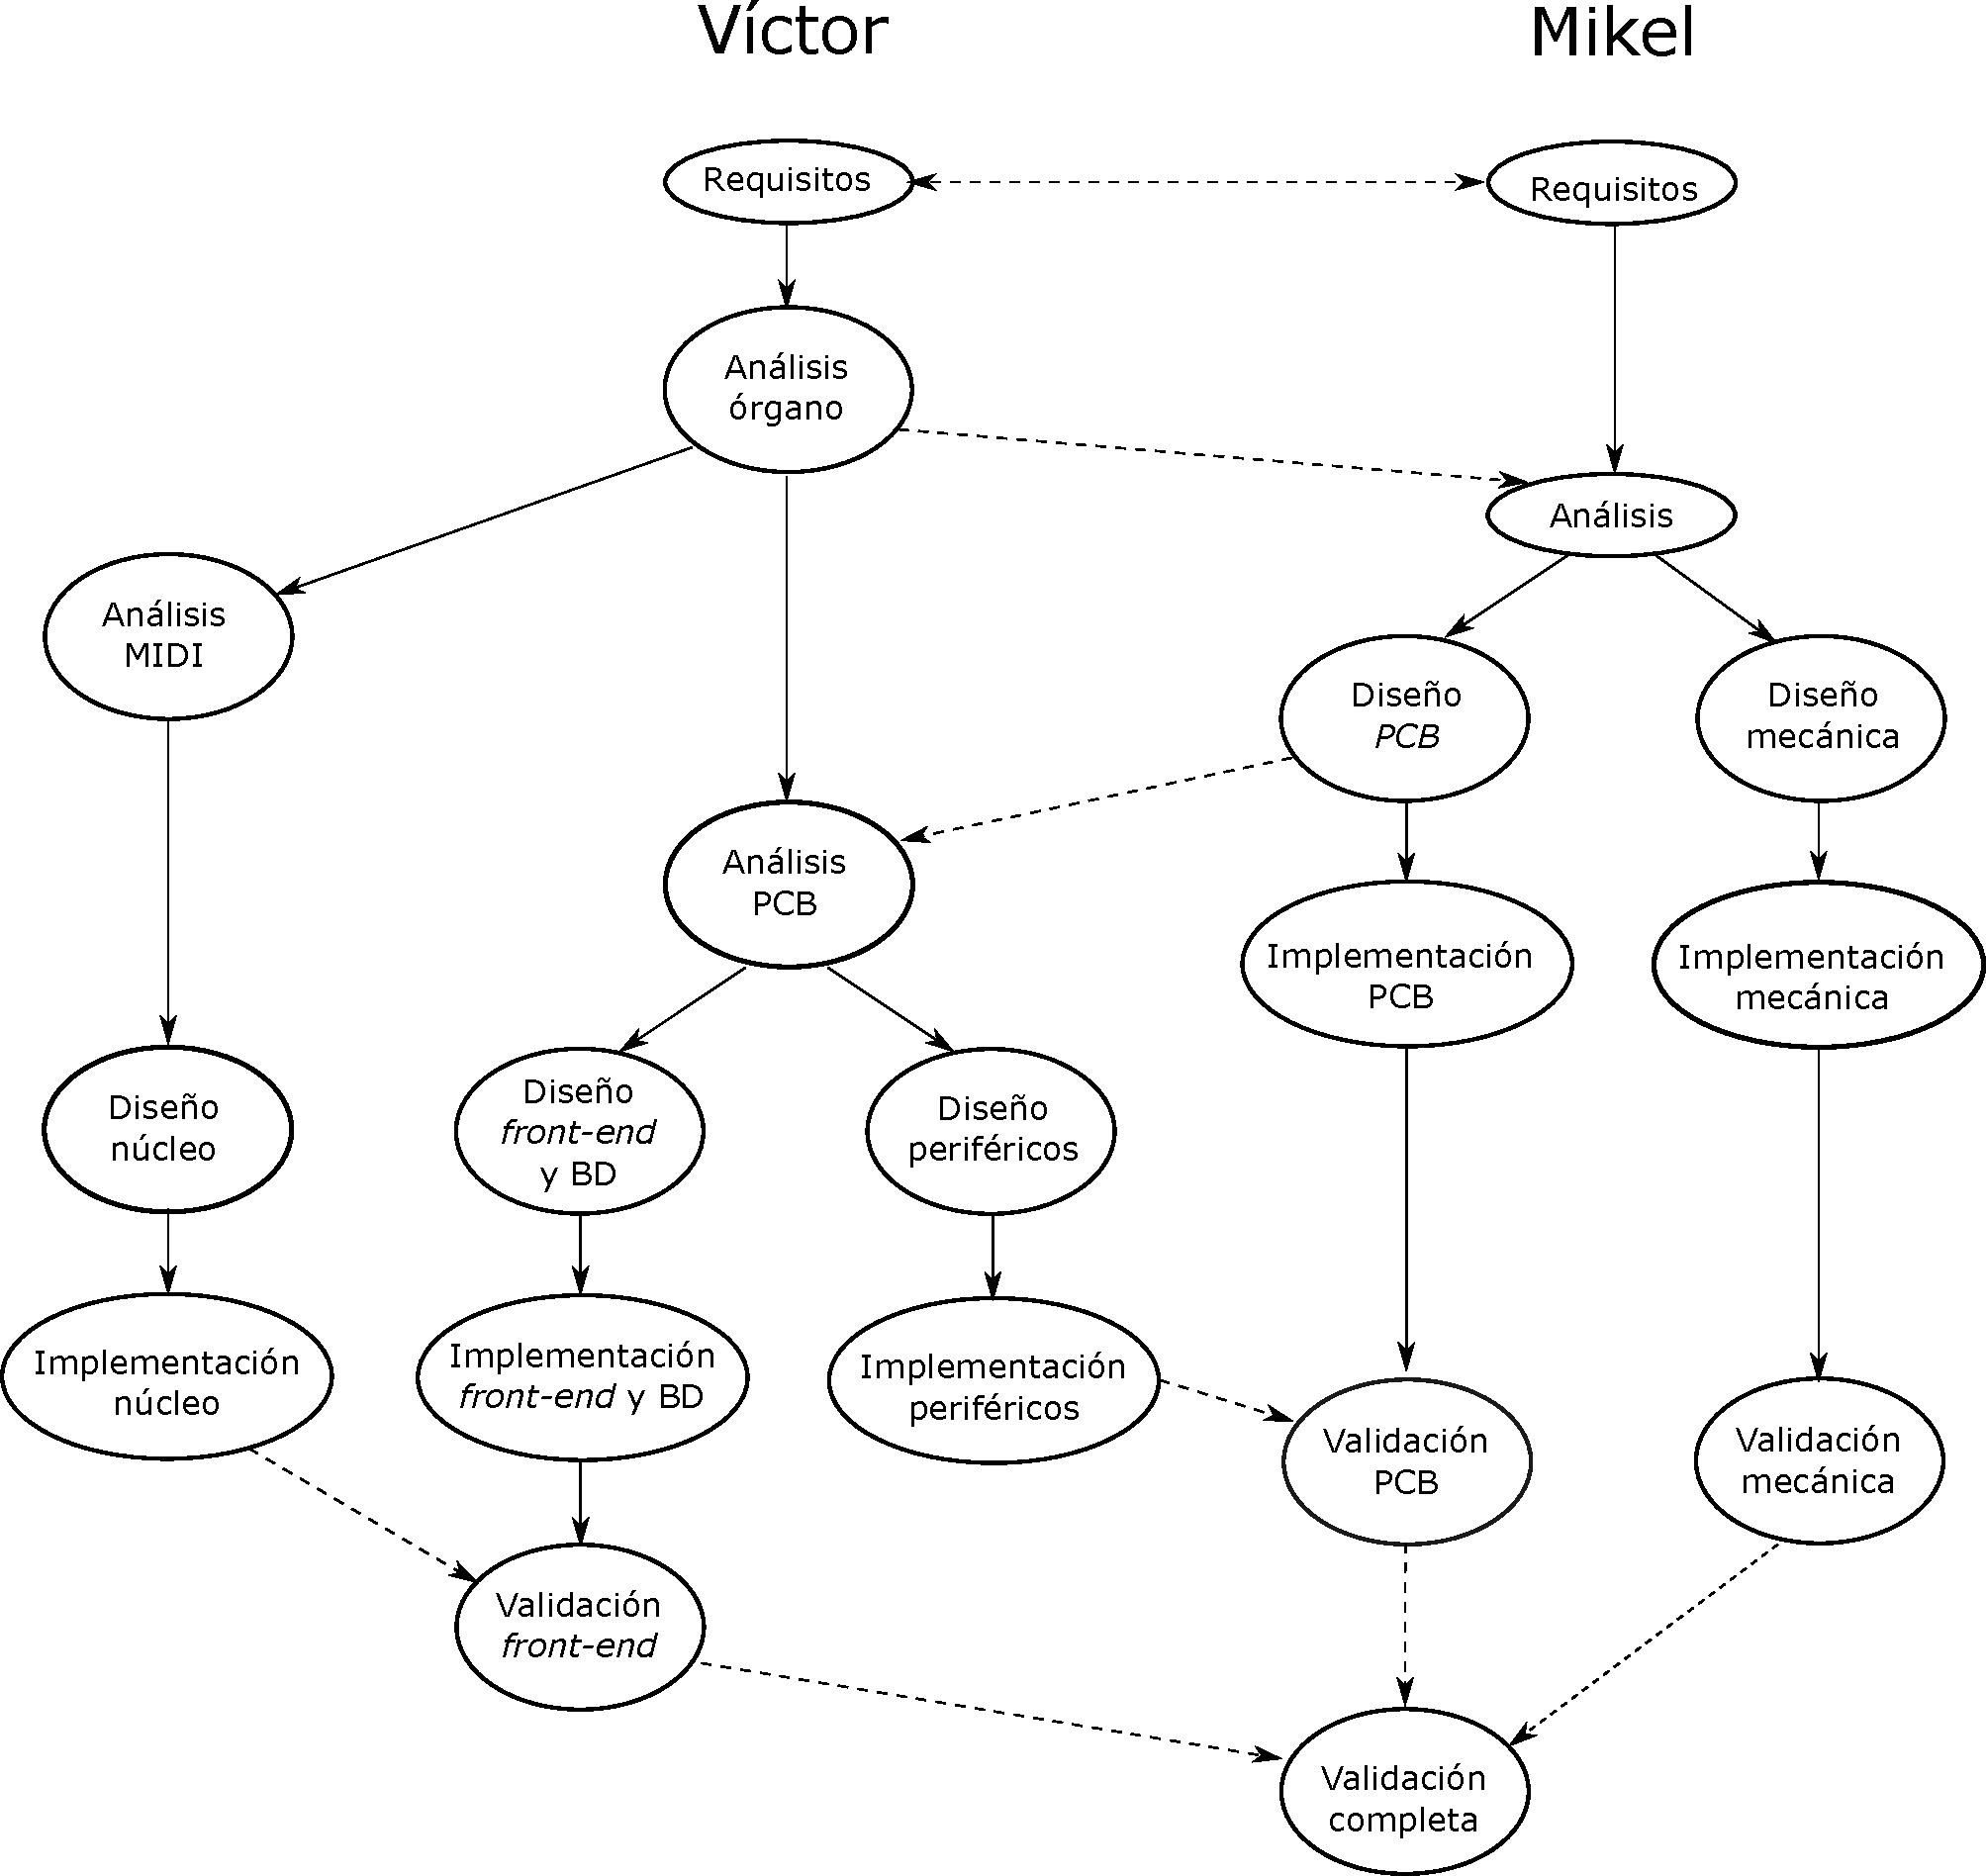
\includegraphics[width=\linewidth]{capitulo2/planificacion}
		\par\end{centering}
	\smallskip
	\caption{\label{fig:planificacion} Diagrama de dependencia de tareas.}
\end{figure} 

\newpage

A la vista de este diagrama, esbozaremos la \textbf{planificación temporal} de esta forma:

\smallskip

\begin{figure}[H]
	\noindent \begin{centering}
		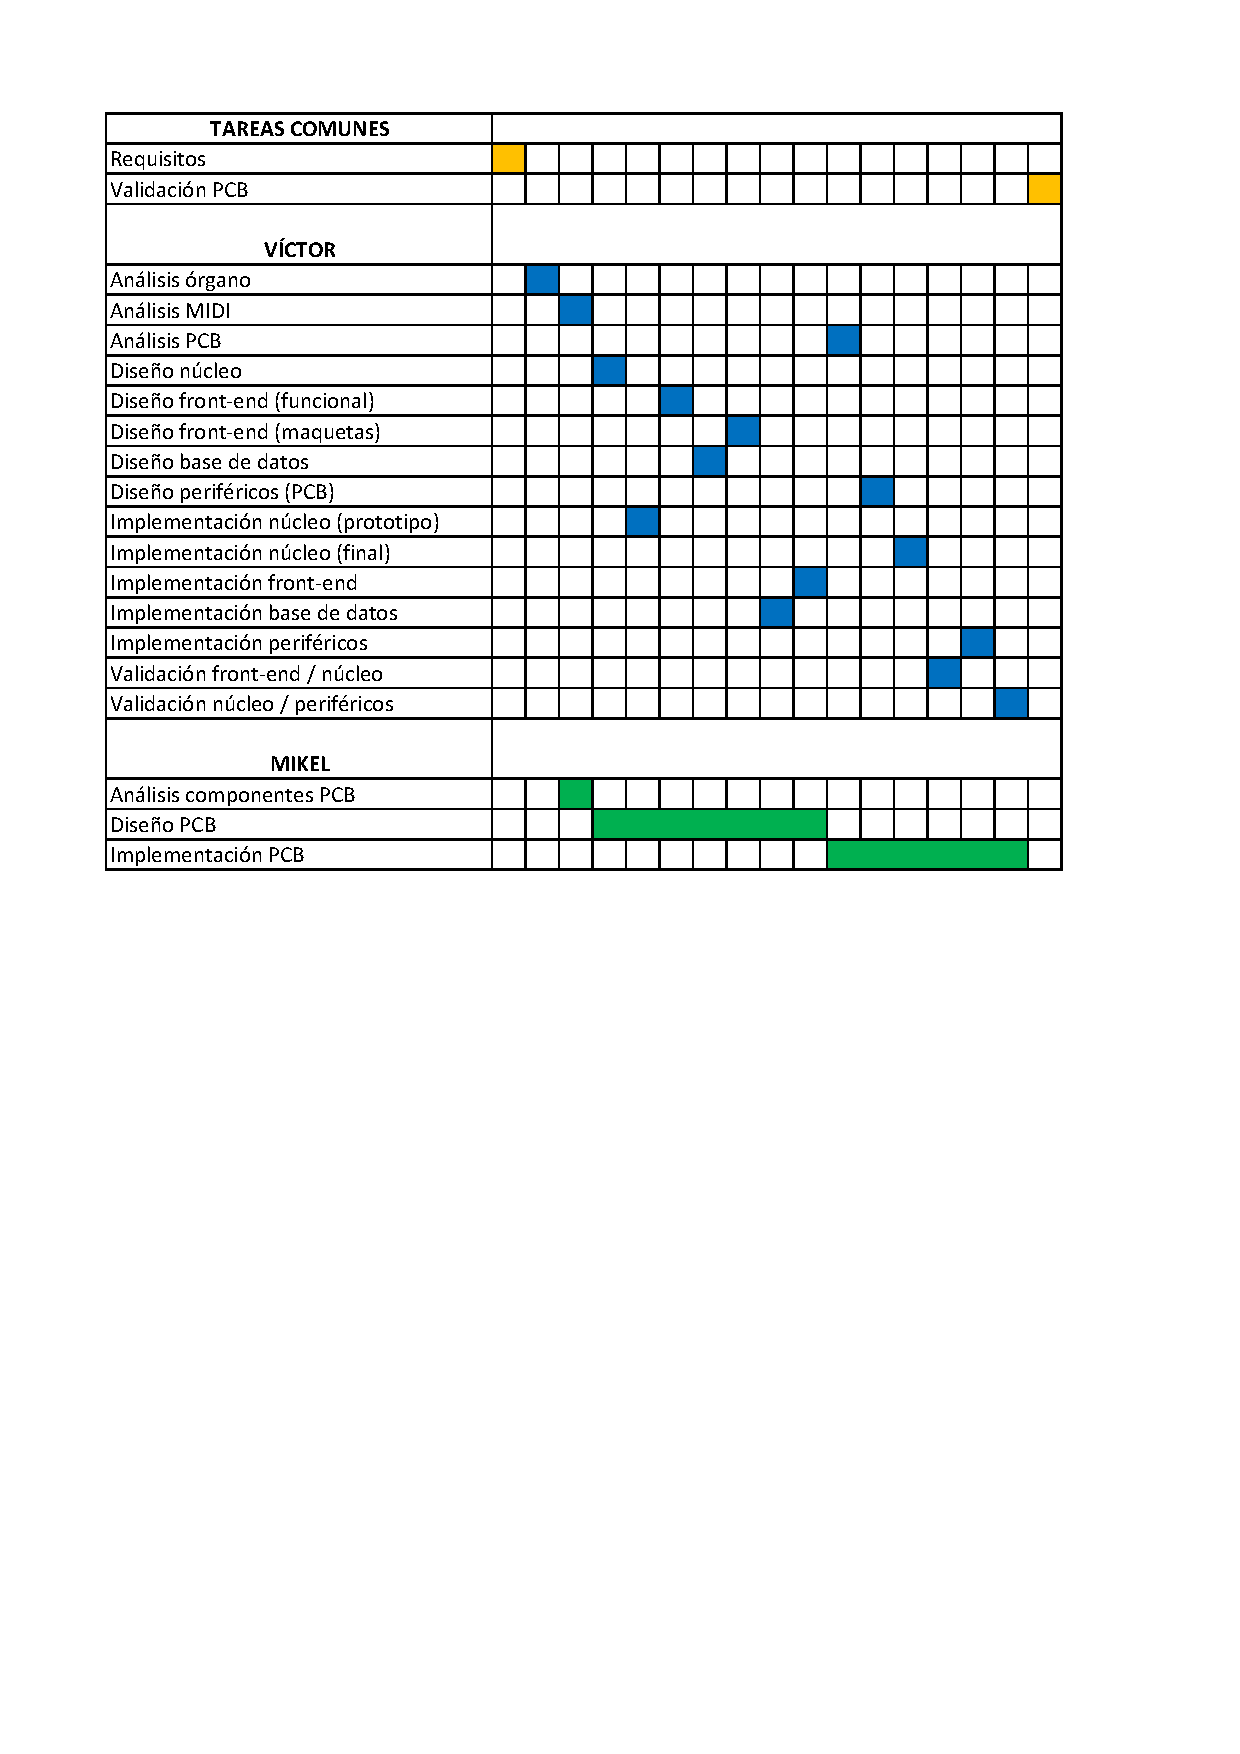
\includegraphics[width=\linewidth]{capitulo2/plan_gantt}
		\par\end{centering}
	\smallskip
	\caption{\label{fig:plan_gantt} Diagrama de Gantt básico.}
\end{figure} 

\smallskip

\subsection{Planificación prevista}

Conocidas las tareas básicas a realizar, proponemos la siguiente planificación para todos los bloques a desarrollar en el sistema. Hemos asignado principalmente las tareas por \textbf{semanas}, aunque algunas de ellas se podrán hacer en común por su simplicidad, y otras deberemos \textbf{descomponerlas} en prototipo e implementación final.

El primer paso es \textbf{analizar} el funcionamiento y la mecánica del órgano para permitir a Mikel continuar su trabajo. Mientras él diseña la \acrshort{PCB}, nosotros comenzamos el \textbf{diseño} de los módulos que no dependen de ésta. Tan pronto como recibamos su diseño, podremos desarrollar el resto del sistema.

\newpage

\begin{figure}[H]
	\noindent \begin{centering}
		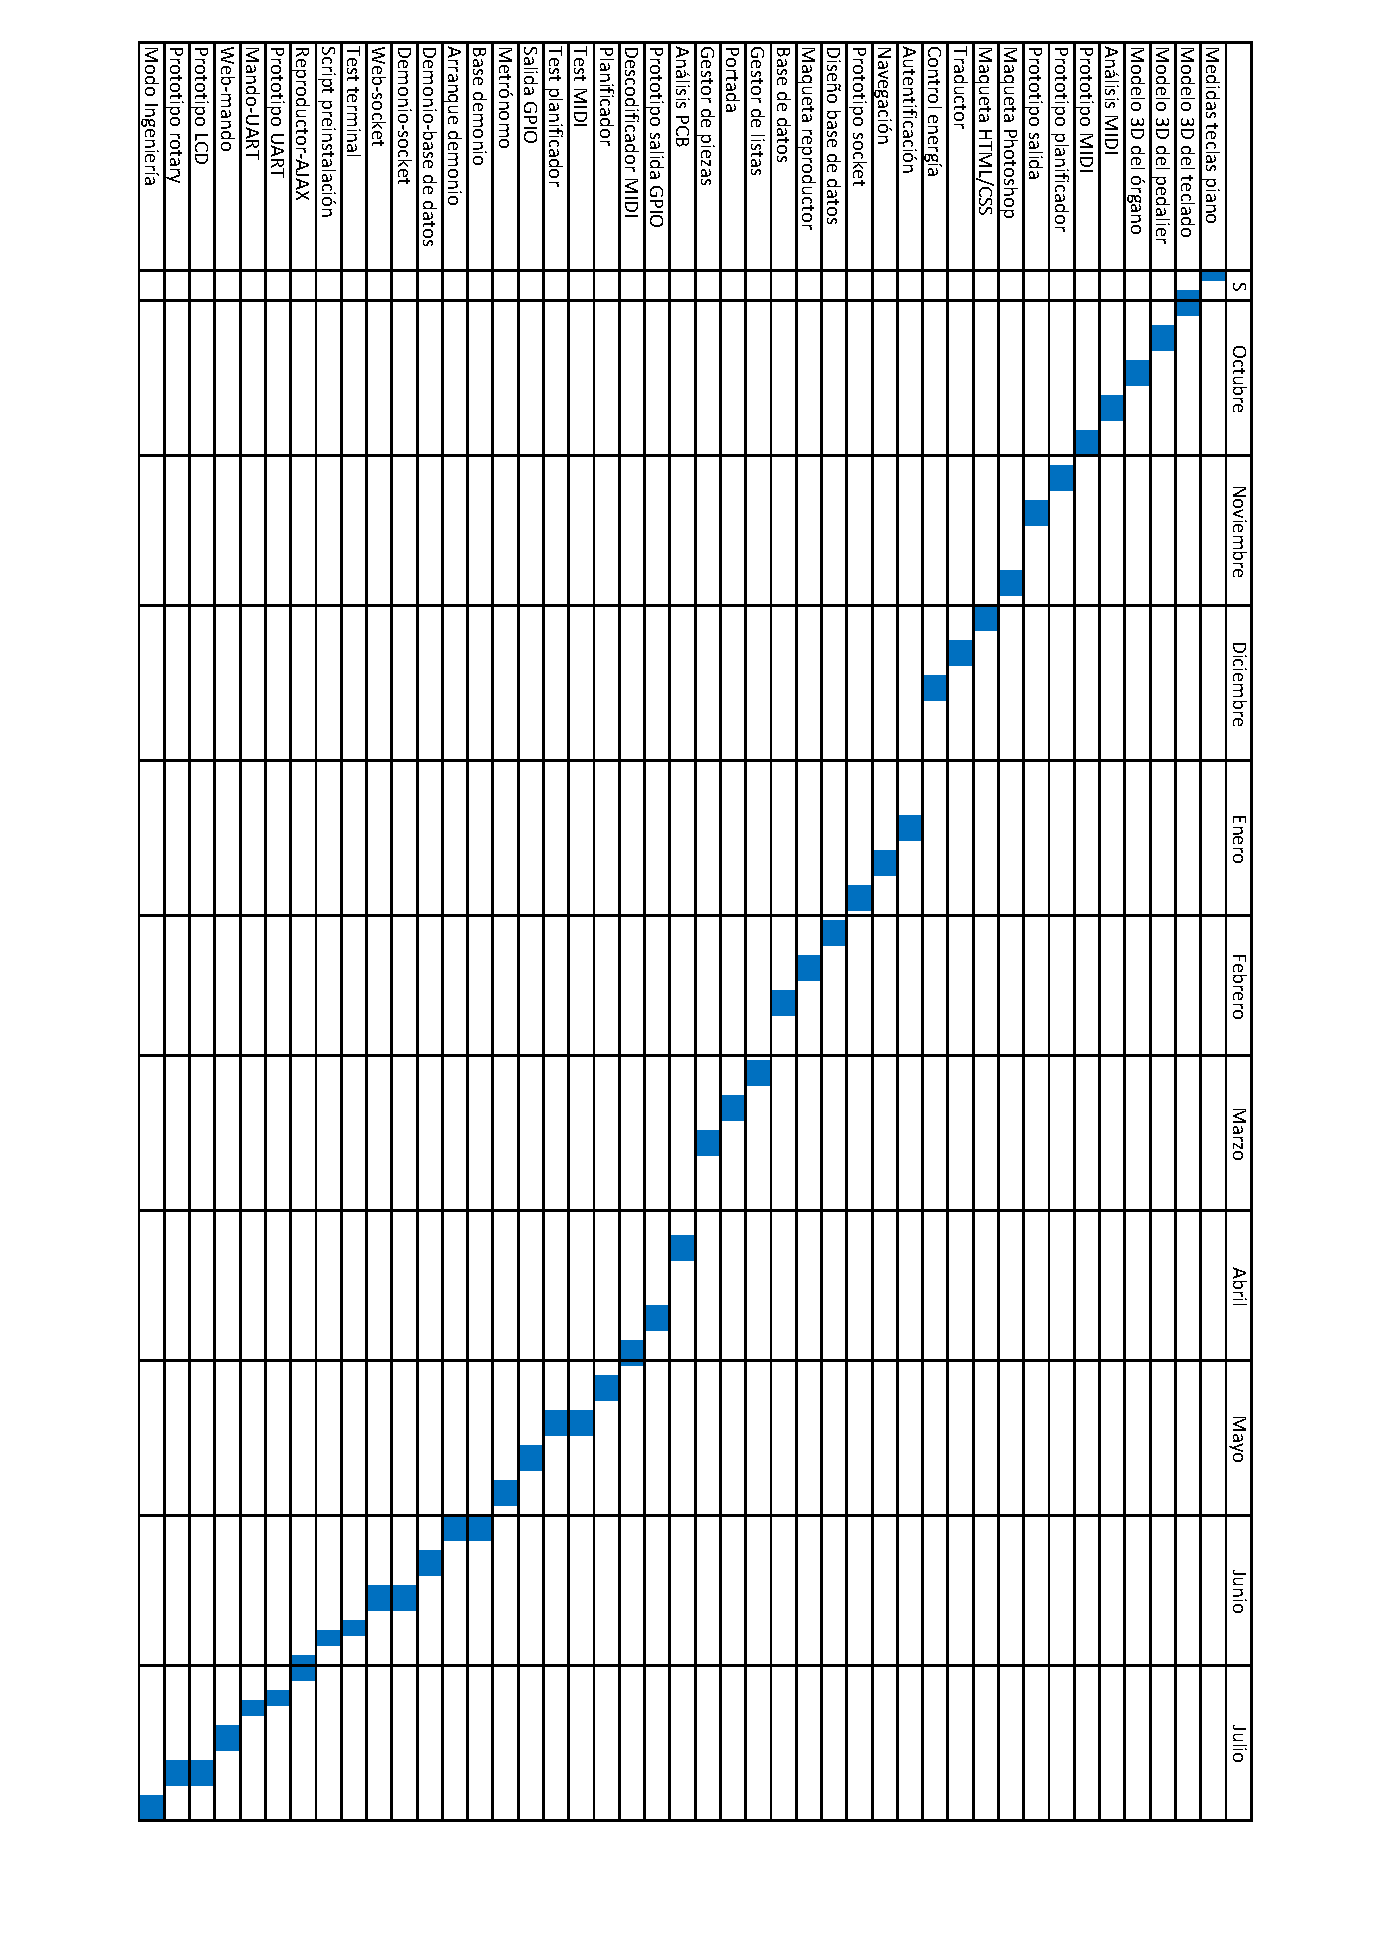
\includegraphics[height=\textheight]{capitulo2/gantt}
		\par\end{centering}
	\smallskip
	\caption{\label{fig:gantt} Diagrama de Gantt para planificación.}
\end{figure} 

\smallskip



\newpage
\clearpage{\pagestyle{empty}\cleardoublepage}
